\documentclass[12pt]{article}

\usepackage{sbc-template}

\usepackage{graphicx,url}

%\usepackage[brazil]{babel}   
\usepackage[utf8]{inputenc}  

\usepackage[T1]{fontenc}
\usepackage{amsmath}
\usepackage{hyperref} 

\usepackage{listings}

% Declare problematic Unicode characters
\DeclareUnicodeCharacter{2248}{$\approx$} % U+2248 is the approximation symbol '≈'


\sloppy

\title{Engenharia de Prompt para Análise Explicável do Comportamento do Motorista usando Dados de Telemetria}

\author{Isaac M. Oliveira\inst{1} Dr. Rafael S. Parpinelli\inst{1} }

\address{Departamento de Computação -- Universidade Federal de Santa Catarina\\
  (UDESC) -- Joinville -- SC -- Brasil
  \email{rafael.parpinelli@udesc.br, isaac.oliveira@edu.udesc.br}
}

\begin{document}

\maketitle

\begin{abstract}
This paper proposes a system for analyzing driver behavior using telemetry data and prompt engineering techniques. Built with Python (Dash and Plotly), the system computes severity scores for events such as speeding and harsh braking. A \textbf{LLM} (Google Gemini) serves as a \textbf{Virtual Driving Instructor}, generating feedback in natural language. The prompt design combines techniques of \textbf{XML structure}, \textbf{Persona}, \textbf{Constitutional AI}, \textbf{Chain-of-Thought}, and \textbf{self-correction}. Based on the literature of \textbf{XAI}, \textbf{DSS}, and \textbf{HCI}, the system improves explainability and user trust.
\end{abstract}

\begin{resumo}
Este artigo propõe um sistema para análise do comportamento de motoristas usando dados de telemetria e técnicas de engenharia de prompt. Construído com Python (Dash e Plotly), o sistema calcula pontuações de gravidade para eventos como excesso de velocidade e frenagem brusca. Uma \textbf{LLM} (Google Gemini) atua como um \textbf{Instrutor Virtual de Direção}, gerando feedback em linguagem natural. O design do prompt combina técnicas de \textbf{XML structure}, \textbf{Persona}, \textbf{Constitutional AI}, \textbf{Chain-of-Thought} e \textbf{self-correction}. Baseado na literatura de \textbf{XAI}, \textbf{SAD} e \textbf{IHC}, o sistema aprimora a explicabilidade e a confiança do usuário. 
\end{resumo}

\section{Introdução}


A segurança no trânsito e a eficiência de frotas dependem fundamentalmente do comportamento do motorista. Sistemas de telemetria hoje registram grandes quantidades de dados de condução – oferecendo oportunidade de identificar comportamentos de risco e instruir motoristas. Na prática, entretanto, gestores de frota frequentemente têm dificuldade em traduzir dados telemétricos em feedback acionável para os motoristas. Mecanismos tradicionais de feedback (por exemplo, pontuações numéricas de risco ou mapas de incidentes) nem sempre são intuitivos ou motivadores para os condutores. Pesquisas mostram que os motoristas preferem explicações textuais de seu desempenho, que fornecem conselhos concretos, em vez de pontuações abstratas ou gráficos. Há uma clara necessidade de relatórios explicativos que façam a ponte entre os dados brutos dos sensores e a compreensão humana, promovendo assim uma condução mais segura e eficiente.

Ao mesmo tempo, avanços recentes em Large Language Models (LLMs) têm permitido que sistemas de IA gerem textos fluentes e contextualizados. LLMs, quando devidamente orientados, podem servir como interfaces de suporte à decisão em linguagem natural que explicam aos usuários insights obtidos a partir de dados. Em domínios de segurança crítica, como a condução, a IA explicável é crucial para a confiança e adoção por parte do usuário. No entanto, usar LLMs para análise de dados telemétricos apresenta desafios: o modelo deve permanecer fiel aos dados, usar um tom apropriado (por exemplo, instrutivo em vez de repreensivo) e evitar ambiguidade ou alucinações. Esses desafios motivam o uso da Engenharia de Prompt – o ofício de projetar prompts de entrada e estratégias de interação para moldar as saídas de um LLM.

Este artigo propõe uma abordagem que combina uma análise de comportamento do motorista baseada em telemetria com técnicas avançadas de engenharia de prompt para produzir explicações de fácil compreensão para condutores. Foi desenvolvida uma aplicação web que recebe dados de condução (arquivos CSV de violações registradas) e calcula um Gravity Score (índice de gravidade) para cada evento com base em regras de negócio configuráveis. Um módulo “Instrutor Virtual” alimentado por um LLM que, a partir dos dados analisados, gera um relatório personalizado de desempenho do motorista. Para garantir que esses relatórios gerados por IA sejam precisos, construtivos e fáceis de analisar, foi elaborado um prompt estruturado com uma persona de especialista, princípios éticos e demonstrações de exemplo embutidos. Técnicas como Constitutional AI (fornecendo ao modelo um conjunto de princípios orientadores), Chain-of-Thought (incentivando raciocínio passo a passo), self-reflection para verificação de erros, e exemplos do tipo few-shot estão integrados ao design do prompt.

O restante deste artigo descreve em detalhes a arquitetura do sistema e a abordagem de engenharia de prompt, e avalia sua eficácia. A Seção 2 revisa os trabalhos relacionados em orientação de motoristas, IA explicável (XAI) e engenharia de prompt. A Seção 3 apresenta a arquitetura do sistema, incluindo o pipeline de processamento de dados e a estrutura do prompt do LLM. A Seção 4 discute os resultados, trade-offs de projeto e feedback dos usuários. Finalmente, a Seção 5 conclui com lições aprendidas e trabalhos futuros para o aprimoramento de sistemas de orientação de motoristas por IA.

\section{Trabalhos Relacionados}

\subsection{Monitoramento do Comportamento do Motorista e Feedback}

O monitoramento do desempenho de motoristas via telemetria tornou-se comum na gestão de frotas. Trabalhos anteriores exploraram modelos de pontuação que correlacionam eventos de condução com risco e eficiência de combustível. Um desafio identificado na literatura é fornecer feedback aos motoristas de forma que influencie a mudança de comportamento. \cite{braun2015} foi pioneiro em gerar feedback textual para motoristas a partir de dados telemétricos, descobrindo que os condutores classificaram esse feedback como mais útil do que painéis contendo apenas pontuações ou mapas. Em um estudo com usuários, 13 de 21 participantes preferiram feedback textual em vez de feedback visual ou numérico para aprender sobre sua condução. Esse estudo também mostrou que explicações textuais deram aos motoristas uma ideia mais clara de como adaptar seu comportamento e foram mais encorajadoras para a melhoria, com efeitos estatisticamente significativos (p \textless{} 0.0001) na percepção de utilidade e motivação. Um sistema subsequente, o SaferDrive \cite{saferdrive2017}, forneceu relatórios semanais de condução gerados automaticamente em linguagem natural e demonstrou uma influência positiva nos hábitos de direção (notadamente reduzindo incidentes de excesso de velocidade) em um teste real. Esses achados ressaltam que feedback explicável e personalizado pode aumentar o engajamento dos motoristas e os resultados de segurança. Este trabalho baseia-se nesse conceito ao usar um LLM moderno para gerar automaticamente feedback de alta qualidade e rico em contexto para motoristas. 

\subsection{IA Explicável em Sistemas de Apoio à Decisão no Transporte}


A explicabilidade é reconhecida como fundamental para sistemas de apoio à decisão em contextos de segurança crítica como o transporte. Na condução autônoma, por exemplo, pesquisadores enfatizam que decisões de IA precisam ser interpretáveis para conquistar a confiança do público. Embora o foco aqui seja a orientação de motoristas humanos (e não a explicação de decisões de veículos autônomos), o princípio subjacente é similar: as partes interessadas necessitam de raciocínio transparente. Sistemas de SAD anteriores para gestão de frotas basearam-se amplamente em gráficos, limiares e alertas baseados em regras, que carecem da clareza narrativa da linguagem natural. Pesquisas em IA explicável indicam que os usuários têm mais probabilidade de confiar e seguir corretamente sugestões de IA quando explicações compreensíveis são fornecidas. Entretanto, explicações ruins ou excessivamente complexas também podem levar a equívocos ou sobrecarregar os usuários. Diretrizes de IHC sugerem que explicações devem ser adaptadas ao contexto do usuário e apresentadas em tom de apoio para serem efetivas. O design do relatório do Instrutor Virtual aproveita esses insights: o relatório é estruturado em seções (visão geral, dicas detalhadas, conclusão) para evitar sobrecarga de informação, e emprega linguagem simples com um tom orientador alinhado às melhores práticas no fornecimento de feedback (por exemplo, destacando pontos positivos e focando em melhorias específicas). 

\subsection{Engenharia de Prompt e Modelos de Linguagem Alinhados}

O surgimento de modelos de LLMs como o GPT-3 e outros permitiu que sistemas de IA fossem programados via prompts em vez de codificação explícita. Engenharia de prompt é o processo de elaborar esses prompts para obter as respostas desejadas. Pesquisadores descobriram várias técnicas para melhorar os resultados dos prompts. O prompting de Chain-of-Thought (CoT) é um método no qual induz-se o modelo a gerar etapas intermediárias de raciocínio, levando a um melhor desempenho em tarefas complexas. Pode-se aplicar CoT incluindo exemplos com raciocínio explícito ou instruindo o modelo a “pensar passo a passo”. \cite{wei2022} mostrou que o uso de CoT nos prompts permite que modelos grandes resolvam problemas de raciocínio de múltiplas etapas com os quais modelos menores ou prompts ingênuos têm dificuldade. No contexto deste trabalho, CoT é relevante para guiar o modelo a analisar logicamente cada infração de condução antes de dar conselhos.

Outra técnica relevante é o prompting com poucos exemplos (\textit{Few-Shot}), em que o prompt inclui alguns exemplos de entrada e saída para ajudar o modelo a generalizar o padrão. \cite{brown2020} demonstrou que, com parâmetros suficientes (por exemplo, o GPT-3 com 175 bilhões de parâmetros), modelos de linguagem tornam-se “aprendizes de poucos exemplos”, capazes de realizar uma tarefa com apenas algumas demonstrações fornecidas no prompt. Essa técnica foi explorada fornecendo um exemplo completo dos dados de um motorista e um relatório bem estruturado no prompt, que serve como um modelo a ser seguido pelo LLM para novos motoristas.

Garantir o alinhamento das saídas do LLM com valores humanos e requisitos da tarefa é outra área ativa de pesquisa. \textit{Constitutional AI}, introduzida por \cite{anthropic2022}, é uma abordagem para alinhar o comportamento da IA por meio de um conjunto de princípios escritos ou uma “constituição” à qual a IA deve aderir. Em vez de (ou além de) aprendizado por reforço com feedback humano, o modelo pode ser guiado por regras explícitas (por exemplo, “a IA não deve fornecer conselhos inseguros”). O prompt inclui tais princípios com foco em comunicação positiva e segura, semelhante a uma constituição para o comportamento de um Instrutor Virtual. Isso se inspira nos resultados da Anthropic que mostram que assistentes de IA guiados por princípios podem ser ao mesmo tempo úteis e inofensivos. De fato,  \cite{bai2022} observou que incorporar raciocínio encadeado no processo de treinamento de uma \textit{Constitutional AI} melhorou tanto o desempenho quanto a transparência das decisões do modelo, alinhando-se ao objetivo de promover raciocínio transparente no feedback.

Por fim, técnicas de autocorreção permitem que um LLM refine sua própria saída. Um exemplo é o método \textit{Self-Refine} \cite{madaan2023}, em que o modelo gera uma resposta inicial, depois a critica e aprimora iterativamente. Tais abordagens têm produzido ganhos de qualidade significativos (modelos como o GPT-4 – \cite{openai2023} – obtendo cerca de 20\% melhores resultados após feedback do próprio modelo). Embora o sistema atual não implemente múltiplas iterações de feedback, foi incorporada uma reflexão mais simples: a saída do LLM é verificada quanto à completude do formato, e o modelo é instruído dentro do prompt a garantir que todas as seções estejam presentes.

\subsection{Prompts Estruturados e Formatação de Saída}

Um desafio prático com sistemas baseados em LLM é garantir que o formato da saída seja correto para uso posterior. Texto livre e não estruturado pode ser ambíguo e difícil de analisar por software. Soluções recentes incluem instruir modelos a produzir saídas estruturadas (por exemplo, JSON ou XML) que possam ser analisadas programaticamente. A OpenAI relata que a engenharia de prompt pura para forçar um formato tinha confiabilidade limitada (cerca de 35\% de sucesso), ao passo que novas ferramentas impondo um esquema podem alcançar 100\% de conformidade de formato. A abordagem proposta, executada antes da disponibilidade do recurso de chamadas de função ou modo de resposta estruturada da OpenAI, utiliza um invólucro em XML projetado manualmente no prompt para organizar o conteúdo.

Ao marcar as seções (persona, princípios, dados, etc.), reduziu-se a ambiguidade na compreensão da tarefa pelo modelo. Sabe-se que o prompting estruturado reduz a variabilidade e os erros nas saídas, facilitando a integração em aplicações. 

Em resumo, este trabalho sintetiza ideias de sistemas anteriores de feedback a motoristas e técnicas modernas de engenharia de prompt. A contribuição deste trabalho inclui um estudo de caso de como o design de prompts pode viabilizar e tornar efetivas explicações de IA em um DSS real.
 
\section{Arquitetura do Sistema}

\subsection{Visão Geral}

O sistema é uma aplicação web que permite aos gestores de frota configurar parâmetros de análise, enviar dados de telemetria, visualizar resultados e gerar um relatório orientado por IA. A arquitetura segue um design modular com um backend de processamento de dados e um frontend interativo. Quando o usuário envia um arquivo CSV de violações, o backend analisa os dados e aplica um conjunto de regras de negócio para calcular uma pontuação de severidade para cada violação e agregar as pontuações por motorista. O frontend, construído com Plotly Dash, exibe várias análises (ranking de motoristas, detalhamento das violações, séries temporais) e fornece uma interface para acionar a geração de relatório pelo LLM. 

\subsection{Pipeline de Dados}

Os registros telemétricos enviados devem seguir um esquema CSV específico. Cada linha representa uma ocorrência de violação (por exemplo, um caso de excesso de velocidade ou uma frenagem brusca). Antes da análise, realiza-se a limpeza dos dados: os nomes das colunas são normalizados, timestamps são convertidos em objetos \textit{datetime}, e quaisquer coordenadas geográficas são transformadas em links de mapa (usando URLs do Google Maps para pontos de início/fim). O sistema pode interpretar tanto valores numéricos quanto \textit{strings} pré-formatadas (por exemplo, coordenadas DMS são convertidas para graus decimais). 

\subsection{Regras de Pontuação de Gravidade}

O cerne da análise de dados é calcular um \textit{Gravity Score} (índice de gravidade) para cada registro de violação (Table 1). Isso é feito por meio de regras configuráveis que codificam conhecimento de domínio sobre risco. Por exemplo, violações de Excesso de Velocidade são segmentadas por contexto: se o limite de velocidade da via (incluído nos dados) é alto (por exemplo, $\ge$ 80 km/h), o evento é tratado como um caso de excesso de velocidade em rodovia; caso contrário, como excesso de velocidade em área urbana ou pátio. São aplicados pesos base diferentes – excesso de velocidade em rodovia tem uma penalidade base maior do que em um pátio privado, refletindo um risco maior. Pontos adicionais são adicionados proporcionalmente ao quanto o veículo excedeu o limite e por quanto tempo. Na configuração padrão adotada, exceder o limite a cada 5 km/h acarreta um incremento (por exemplo, 0,2 pontos por 5 km/h acima, dobrando para 0,4 pontos se a velocidade ultrapassou 100 km/h), e cada 10 segundos de duração acrescenta mais 0,1 ponto. Assim, um incidente prolongado e extremo de excesso de velocidade acumulará uma pontuação alta, ao passo que um excesso breve e leve pode resultar em pontuação baixa. Outras violações como Frenagem Brusca têm regras mais simples – um peso base fixo (por exemplo, 0,1), já que qualquer ocorrência é um evento de segurança mas não há componente de duração. RPM Excessiva e Marcha Lenta (rotulados “RPM excessiva” e “Marcha lenta”) usam pontuação baseada em duração: quanto mais tempo o motor ficou em alto RPM ou estado de marcha lenta além dos limiares, mais pontos são atribuídos. Esses parâmetros podem ser ajustados via a UI para se adequar às políticas específicas de uma frota ou a novos insights. 


\begin{table}[h!]
    \centering
    \caption{Tipos de Violação e Parâmetros Padrão}
    \label{tab:violation_types_pt} % Alterado o label para refletir a tradução
    \tiny % Mantendo o tamanho da fonte pequeno
    \setlength{\tabcolsep}{3pt} % Mantendo a separação de colunas reduzida
    \begin{tabular}{|l|p{2.5cm}|c|p{4cm}|} % Mantendo larguras ajustadas para quebra de texto
        \hline
        \textbf{Tipo de Violação} & \textbf{Descrição} & \textbf{Peso Base} & \textbf{Fatores Adicionais} \\
        \hline
        Velocidade Excessiva – Rodovia & Excesso em rodovia ($>$80km/h) & 0,2 & +0,2 por 5km/h acima; +0,4 se $>$100; +0,1 por 10s \\
        Velocidade Excessiva – Serra & Excesso em serra ($\le$80 $>$40) & 0,1 & +0,1 por 5km/h; +0,2 se $>$65; +0,05 por 10s \\
        Velocidade Excessiva – Pátio & Excesso em pátio ($\le$40km/h) & 0,1 & +0,1 por 5km/h; +0,05 por 10s \\
        Marcha Lenta & Motor ligado parado & 0,1 & +0,1 por 20min; eventos $<$10min ignorados \\
        Freada Brusca & Redução rápida de velocidade & 0,1 & (Sem fator de duração) \\
        RPM Excessiva & RPM acima do ideal & 0,07 & +0,07 por 30s acima do limite \\
        Faixa Verde & Fora da faixa ideal de RPM & 0,07 & +0,07 por 3min fora da faixa \\
        Freio Motor & Uso excessivo do freio motor & 0,07 & +0,07 por 2min sustentados \\
        \hline
    \end{tabular}
\end{table}

\subsection{Módulo Instrutor Virtual}


As pontuações por evento são então agregadas. A pontuação total de cada motorista é a soma das pontuações de suas violações. O sistema produz um ranking de motoristas por pontuação total (maior implica mais risco). Adicionalmente, são computadas estatísticas resumidas como total de eventos por tipo e contribuição de risco por categoria (segurança vs. economia). Isso é exibido no \textit{dashboard} e também alimentado no prompt do LLM para destacar os problemas mais significativos de cada motorista.

O destaque do sistema é o Instrutor Virtual – um agente de IA que produz um relatório narrativo para um motorista selecionado. Quando o usuário seleciona um motorista e clica em “Gerar Relatório”, o sistema monta um prompt para o LLM. Esse prompt é cuidadosamente construído para incluir: uma definição do papel da IA (uma persona de instrutor de direção), um conjunto de princípios de \textit{coaching}, um esboço do formato requerido do relatório, um ou mais relatórios de exemplo e, por fim, os dados específicos do motorista (sua pontuação total e detalhes-chave das violações). O LLM recebe esse prompt e retorna um relatório formatado em Markdown. O relatório normalmente começa com uma saudação personalizada, traz uma avaliação geral do desempenho do motorista, então enumera algumas principais áreas problemáticas com explicações e dicas, e finaliza com uma recomendação ou incentivo final.

Utiliza-se a API da IA Generativa do Google para essa tarefa. O modelo Gemini utilizado (v1.5) \cite{google2023} é um modelo de linguagem de grande porte multilíngue capaz de entender a estrutura do prompt e produzir saídas fluentes em português. A API é chamada com parâmetros ajustados para uma saída relativamente determinística (\textit{temperature ≈ 0,4}, \textit{top-P} = 1) a fim de garantir consistência. A resposta do modelo é capturada pela aplicação e exibida em uma área de texto para o usuário. O usuário pode editar esse texto, se necessário (por exemplo, um gestor pode ajustar a formulação ou adicionar notas específicas da empresa) e então o relatório pode ser exportado como um arquivo HTML para impressão ou compartilhamento.


\subsection{Implementação da Engenharia de Prompt}

\begin{figure}[ht]
\centering
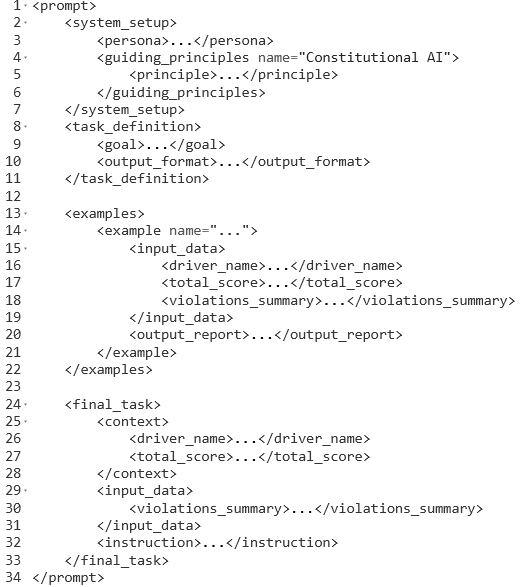
\includegraphics[width=.4\textwidth]{prompt_black_white.png}
\caption{Estrutura de exemplo}
\label{fig:exampleFig1}
\end{figure}

A construção do prompt para o LLM é central para o sucesso do sistema. Foi implementada uma função \verb|get_virtual_instructor_prompt_template()| no código, que retorna um \textit{template} com múltiplas seções. Esse \textit{template} usa uma estrutura semelhante a XML para maior clareza. As principais seções do prompt são:

\begin{itemize}
    \item \verb|<system_setup>|: Esta seção estabelece o contexto para o LLM. Dentro dela:
    \begin{itemize}
        \item \verb|<persona>|: Aqui explicita-se ao modelo que ele é um “Instrutor Virtual de Direção, especialista em gestão de frotas e análise de telemetria”, com a missão de orientar motoristas. Isso prepara o modelo para adotar um tom de autoridade, porém prestativo.
        \item \verb|<guiding_principles name="Constitutional AI">|: Nesta seção, listam-se quatro princípios que o modelo deve seguir. Estes são efetivamente a “constituição” para as respostas da IA. Em resumo, os princípios dizem: (1) Basear o feedback estritamente nos dados fornecidos (evitar suposições); (2) Manter um tom de apoio e construtivo – focar na melhoria, não na culpa, e usar linguagem respeitosa; (3) Dar recomendações práticas e acionáveis ligadas aos eventos; e (4) Priorizar a segurança acima de tudo, enfatizando a prevenção de acidentes.
        \item \verb|<task_definition>|: Esta seção explica o que se deseja que a IA faça. Especifica-se o objetivo (“Gerar um relatório de melhoria de direção...”, ou seja, um relatório individual de aperfeiçoamento na condução) e uma descrição do formato de saída. O formato de saída é dado como uma lista numerada de seções: (1) Análise Geral – saudação e resumo com a pontuação total; (2) Pontos de Melhoria Detalhados – explicações das violações mais significativas, com contexto de risco e dica prática para cada uma, incluindo o link do mapa; (3) Recomendação Final – uma “dica de ouro” conclusiva baseada no padrão geral.
    \end{itemize}
    \item \verb|<examples>|: Fornece-se um exemplo concreto dentro do prompt. Devido a restrições de comprimento do prompt, foi incluído um exemplo (chamado “Análise para João Silva”). Nesse exemplo:
    \begin{itemize}
        \item \verb|<input_data>| fornece um nome de motorista fictício “João Silva”, um \verb|total_score| de 85.00, e uma lista \verb|violations_summary| com uma violação de exemplo. A violação listada é um evento de excesso de velocidade (30 pontos) com data/hora, duração e um link de mapa.
        \item \verb|<output_report>| fornece um relatório de exemplo correspondente àquela entrada. O conteúdo mostra como se espera que o modelo escreva: ele cumprimenta João, observa em linhas gerais que alguns pontos precisam de atenção, então, sob uma subseção “Pontos de Melhoria com Contexto”, descreve em detalhe a violação de excesso de velocidade, incluindo explicação do risco, dicas práticas e informações de localização. Esse exemplo é crucial – demonstra o tom desejado (note que diz “Olá, João!” de maneira amigável, e então mantém um tom encorajador) e o formato (todas as seções presentes, seções usam títulos Markdown apropriadamente, dicas estão em itálico ou em forma de lista, etc.). Ao incluir isso no prompt, o modelo tem uma referência de estilo e estrutura que deve emular. Isso é efetivamente um aprendizado com poucos exemplos (\textit{few-shot}): o modelo vê um par de entrada–saída (ou poderia ver alguns) e aprende a produzir uma saída similar para novas entradas.
    \end{itemize}
    \item \verb|<final_task>|: Após o exemplo, o prompt termina com a tarefa específica para o motorista atual. São então fornecidos o \verb|<driver_name>| e \verb|<total_score>| reais do motorista selecionado, bem como o \verb|<violations_summary>| montado dele (que pode ter 1–3 principais violações). Por fim, uma \verb|<instruction>| diz explicitamente ao modelo para “executar a análise e gerar o relatório para o motorista especificado, seguindo estritamente o formato e as diretrizes”. Essa instrução reforça que agora ele deve aplicar tudo acima para produzir uma nova saída.
\end{itemize}
O prompt inteiro é delimitado por uma tag de nível superior \verb|<prompt>| para sinalizar o início e fim. Observou-se que usar tags XML (ou quaisquer tokens distintivos) para cada parte tornou mais fácil verificar ou extrair partes, se necessário, e provavelmente ajuda o modelo a diferenciar entre instrução, exemplo e dados.




\subsection{Autoverificação e Pós-processamento}

Após chamar a API, o sistema verifica a resposta. Se o modelo retornar conteúdo na estrutura esperada (que deve ser Markdown com as seções), a resposta é aceita. Realizou-se uma validação mínima: assegurando que o texto não está vazio e contém certas palavras-chave que indicam que cada seção está presente (por exemplo, “Análise Geral”, “Pontos de Melhoria” e “Recomendação Final”). Se algo estiver errado (por exemplo, o JSON da API não possui candidatos, ou o conteúdo não está como esperado), o código registra um erro e retorna uma mensagem como “Não foi possível gerar a análise”. 

Por fim, o relatório em Markdown é renderizado na interface web. O usuário poderá editá-lo livremente após revisão. Também foi fornecida uma função de Exportar que pega indicadores-chave de desempenho e produz um arquivo HTML (para download). O HTML inclui, por exemplo, algumas estatísticas resumidas (total de eventos, pior dia, etc.) e o texto gerado. Isso permite que a saída seja compartilhada com os motoristas (por exemplo, via e-mail ou mensagem de texto).

\section{Discussão}

\subsection{Efetividade da Engenharia de Prompt em Sistemas de Apoio à Decisão}

Este projeto ilustra que uma engenharia de prompt cuidadosa pode transformar um LLM visto como caixa-preta em um consultor específico de domínio. Ao investir esforço no prompt (que atuou como um pequeno roteiro de sistema especialista), foi possível alcançar um comportamento do modelo que de outra forma exigiria extenso \textit{fine-tuning} ou programação baseada em regras. O Instrutor Virtual efetivamente codifica uma combinação de conhecimento de especialista (por meio do exemplo e dos princípios) e personalização orientada por dados (por meio da inserção das métricas reais do motorista). Essa abordagem híbrida – combinando regras escritas por humanos (no prompt) com texto gerado por ML – mostrou-se poderosa. Ela demonstra um modo prático de obter uma saída de IA explicável sem precisar que o modelo explique inerentemente seu próprio funcionamento interno.


\subsection{Aceitação e Confiança do Usuário}

O feedback positivo dos usuários indica que a explicabilidade melhora tangivelmente a aceitação pelos usuários. Os motoristas mostraram-se mais dispostos a se engajar com o feedback quando este estava em uma forma narrativa amigável. Os gestores encontraram valor nos relatórios de IA como complemento à sua própria expertise, e não um substituto. Isso sugere que explicações de IA em domínios de condução veicular podem aprimorar, em vez de substituir, o julgamento humano quando projetadas adequadamente. A principal percepção é que a IA serve como uma “assistente de coaching” que fornece feedback estruturado e consistente, enquanto os humanos mantêm a capacidade de contextualizar, modificar e entregar a mensagem pessoalmente. Essa abordagem híbrida humano-IA aproveita as forças de ambos: a capacidade da IA de processar grandes quantidades de dados e gerar explicações consistentes, e a capacidade humana de entender o contexto, construir relacionamentos e adaptar o estilo de comunicação. 


\section{Conclusão e Trabalhos Futuros}


Várias limitações da abordagem atual sugerem direções para trabalhos futuros. Primeiro, a abordagem de engenharia de prompt adotada, embora efetiva, é um tanto frágil – mudanças no modelo de LLM ou na API poderiam requerer ajustes no prompt. Abordagens mais robustas podem envolver realizar o \textit{fine-tuning} de um modelo especificamente para este domínio. Segundo, a avaliação conduzida limitou-se a um único conjunto de dados e a um estudo de usuários relativamente pequeno. Uma implantação em maior escala forneceria mais insights sobre a efetividade a longo prazo e o potencial de mudança de comportamento. Terceiro, o sistema atual gera relatórios para motoristas individuais, mas insights em nível de frota e análises comparativas poderiam ser valiosos. Trabalhos futuros poderiam explorar a geração de relatórios para toda a frota que identifiquem padrões comuns e sugiram melhorias sistêmicas.

Adicionalmente, o sistema foca em feedback reativo (analisando violações passadas). Uma abordagem mais proativa poderia envolver \textit{coaching} em tempo real ou análise preditiva para prevenir violações antes que ocorram. Isso exigiria integração com fluxos em tempo real e, possivelmente, modelos de aprendizado de máquina mais sofisticados para predição. Em suma, este estudo demonstrou o potencial de integrar LLMs alinhados ao contexto de telemetria veicular para aprimorar a segurança e a eficiência na condução, embora haja espaço para aprimorar a robustez e a escalabilidade dessa abordagem em desenvolvimentos futuros.


\bibliographystyle{sbc}
\bibliography{sbc-template}

\end{document}
